\iffalse
\documentclass[DIV=15]{scrartcl}


\usepackage[demo]{graphicx}
\usepackage{epstopdf} 
\usepackage{url,amsfonts,amsmath,enumerate,amssymb,bm,siunitx,xcolor,soul}
\usepackage[numbers]{natbib}
\usepackage{tabularx}  % for 'tabularx' environment and 'X' column type
\usepackage{ragged2e}  % for '\RaggedRight' macro (allows hyphenation)

\usepackage[font=small]{caption}
\usepackage[labelformat = empty,position=top]{subcaption}
\usepackage[export]{adjustbox}


\newcolumntype{Y}{>{\RaggedRight\arraybackslash}X} 


\begin{document}
\fi







%%%%%%%%%%%%%%%%%%%%%%% file template.tex %%%%%%%%%%%%%%%%%%%%%%%%%
%
% This is a general template file for the LaTeX package SVJour3
% for Springer journals.          Springer Heidelberg 2006/03/15
%
% Copy it to a new file with a new name and use it as the basis
% for your article. Delete % signs as needed.
%
% This template includes a few options for different layouts and
% content for various journals. Please consult a previous issue of
% your journal as needed.
%
%%%%%%%%%%%%%%%%%%%%%%%%%%%%%%%%%%%%%%%%%%%%%%%%%%%%%%%%%%%%%%%%%%%

%
%\documentclass[natbib]{svjour3}                     % onecolumn (standard format)
%\documentclass[smallextended]{svjour3}     % onecolumn (second format)
\documentclass[twocolumn]{svjour3}         % twocolumn
%
\smartqed  % flush right qed marks, e.g. at end of proof
%

\usepackage{graphicx}
\usepackage{floatrow}
\usepackage{subfig}

\usepackage{epstopdf} 
\usepackage{url,amsfonts,amsmath,enumerate,amssymb,bm,siunitx,xcolor,soul}
\usepackage[numbers]{natbib}
\usepackage{tabularx}  % for 'tabularx' environment and 'X' column type
\usepackage{ragged2e}  % for '\RaggedRight' macro (allows hyphenation)
\newcolumntype{Y}{>{\RaggedRight\arraybackslash}X} 
%
\usepackage{mathptmx}      % use Times fonts if available on your TeX system
% \usepackage{chicago-bibstyle}  % use this style if you don't use BibTeX.
%
% insert here the call for the packages your document requires
%\usepackage{latexsym}
% etc.
%
% please place your own definitions here and don't use \def but
% \newcommand{}{}
%
% Insert the name of "your journal" with
% \journalname{myjournal}
%
% Definitions for the journal names
\newcommand{\aap}{{Astron. Astrophys.}}
\newcommand{\apj}{{Astrophys. J.}}
\newcommand{\grl}{{Geophys. Res. Lett.}}
\newcommand{\solphys}{{Solar Phys.}}
%
\begin{document}

\title{Insert your title here%\thanks{Grants or other notes
%about the article that should go on the front page should be
%placed here. General acknowledgments should be placed at the end of the article.}
}
\subtitle{Do you have a subtitle?\\ If so, write it here}

%\titlerunning{Short form of title}        % if too long for running head

\author{First Author         \and
        Second Author %etc.
}

%\authorrunning{Short form of author list} % if too long for running head

\institute{F. Author \at
              first address \\
              Tel.: +123-45-678910\\
              Fax: +123-45-678910\\
              \email{fauthor@example.com}           %  \\
%             \emph{Present address:} of F. Author  %  if needed
           \and
           S. Author \at
              second address
}

\date{Received: date / Accepted: date}
% The correct dates will be entered by the editor


\maketitle

\begin{abstract}
%real  params  transmission of resistance tonot on prep $20\%$ DRAMS $25\%$ chateauof WT  parnters $75\%$ reduction in incidence mutation rate of $(5e-5)$ means  there is more resistance than when it  is  $(5e-5)^2$ changing time to art from 1  to 1.5 not makle much differencec.

\newpage


The only bit that I think might be ‘wrong’, or at least needs more thinking about, is the mutation rates used.  If resistance requires 2 mutations (because there are two drugs), then you could argue that the probability of evolving resistance is $2.5 x 10^-9$. You could probably make an argument that for now you ignore single mutations because they carry a fitness cost but don’t make you resistant, so in all situations they are selected against.

Some main points:

Make sure every sentence is explicit.  Don’t leave any space for ambiguity.
The model itself need much more time spent on explaining it, what the implicit and explicit assumption are etc.  At the moment it is very difficult to follow.
When presenting the model, start with the simple case of good adherence, then add poor adherence (I didn’t really understand the poor adherence bit).

poor adherence make itmeans iinfection more likely and emergence of resistant also more likely



Maybe a figure of the profile of HIV infection might be helpful.
Add a table given all variables and parameters and the values where appropriate, with references.  Otherwise the reader is lost.
Make sure you discuss what is next eg.
assumptions that need relaxing
More realistic fitness landscape – model resistance to both strains explicitly and compensatory mutations
Testing more stuff
Testing with a simulation
Etc.

Other thoughts.  The discussion on whether to include homeostatic proliferation is a bit tangential.  I would simply choose a set of parameters and explore what we are more interested in a bit more thoroughly e.g.. Transmission from the reservoir, competition at the point of transmission, cost of resistance, and so on.

\newpage

HIV causes significant morbidity and mortality  worldwide. Despite the availability  of drugs that can significantly reduce viral load allowing people to remain relatively healthy, there is no way to eradicate the virus entirely from their body.  A preventative strategy that can be employed in at risk people is to give them a subset of   the antiviral drugs used to treat HIV infection. With high adherence, this massively reduces the chance of acquiring he virus, but sub-optimal adherence can lead to the emergence  of drug resistant strains  which may then be transmitted.   The potential for transmitted drug resistance might further be exacerbated by the presence of a reservoir of infected cells which  forms soon after infection. The reservoir is long-lived and importantly the virus does not actively replicate in these cells and so is not affected by the antiviral drugs. When the drugs are no longer being taken,  activation of cells in the reservoir can restart infection.   Due to the reservoir these strains may be able to persist for a long time, potentially increasing the risk of developing resistance  to HIV treatment. We show that the transmissibility of resistamtn strains is  low thsre is not asuch a porlem ???????

low transmissibility

 the use of  PrEP is unliely  toincreases the incidence of  tranismisitted infections    
\keywords{First keyword \and Second keyword \and More}
% \PACS{PACS code1 \and PACS code2 \and more}
% \subclass{MSC code1 \and MSC code2 \and more}
\end{abstract}



\section{Introduction}
\label{intro}




%from van de vijer:                      Daily oral preexposure prophylaxis (PrEP) with tenofovir and emtricitabine can prevent $44–75\%$ of new HIV infections \cite{iprex2011} [2–4]. Two studies [5,6] have found no protective effect of PrEP on prevention



HIV is a major health problem around  the world~\cite{unaids} and cure still seems to be along way off~\cite{passaes2014} and therefore there is intense effort in designing strategies to prevent its spread(REF). A promising strategy for at risk individuals is the use of pre-exposure prophylaxis (PrEP). The antiretroviral treatment (ART) for HIV consists of a combination of drugs that each inhibit viral replication  in different ways (REF). The idea of PrEP is that by taking these drugs uninfected individuals  reduce their chances of infection. 
The most commonly used  drugs in PrEP are the reverse transcriptase inhibitors  tenofovir and emtricitabine (REF), resistance to each of these  is due to a single point mutation (REF). The rate at which the HIV virus mutates and replicates means that even for a moderate viral load  every single point mutation will occur thousands of times a day~\cite{coffin1995}.  % and maybe even every double mutation (REF).                                    
A key concern of researchers is that  PrEP might  be inadvertently selecting for viral  strains that will be more resistant to ART(RFE?). There have been several large studies looking into the effectiveness of PrEP~\cite{iprex2011,partners2012}(MORE). With high levels of  adherence about  $90\%$ of HIV infections can be avoided~\cite{iprex2011,partners2012}  for serdiscotant africa n hetersexual couples bu for agayes is differetn in thebum. Analysis of the data  generated has shown that the emergence of resistance (to either drug used) is rare and mostly happens when the individual had an undetected HIV infection prior to taking PrEP(REF). Because of this risk HIV tests are taken before going onto PrEP, the most common (and cheapest) of which are antibody tests(REF). However  these only work after seroconversion, the time at which the body produces HIV specific antibodies.  The results also take some  time to be available,  there are better tests which can detect much earlier infection, such as looking for viral RNA. These are more expensive  and would add a significant cost to any wide scale   PrEP regime(REF).
  %which occurs SOME TIME AFTER INITIAL INFECTION (REF). 
 %Checking for HIV antibodies common test, but need to wait for immune system to respond about a month should be enough for most people but it can take longer to detect. Direct tests are quicker, e.g. detect proteins associated with HIV, this can detect virus usually within 10-14 days after infection. levels of this protein (p24) decrease after five to six weeks and can not be detected.  Or can look for viral RNA in blood, this can detect virus as early as  7 to 14 days after infection Depending on the type of test used  it can take several months for the virus to be detected(REF).
 An important question is whether the benefit of reducing infections is worth the cost of increasing the amount of  resistant virus.
  The effectiveness of PrEP at preventing transmission has been borne out by most trials  (REF), but the long term effects are not yet known. Several  modelling studies have shown that  ART drives the development of resistance more than does PrEP and that poor adhernce/ineffective PrEP leads to more HIV infections but there is less  selective pressure for the emergence of  resistance~\cite{abbas2013}(MORE REF). An important drawback of these models is that they do not explicitly account for the within host dynamics, although this can have a large influence on the evolutionary dynamics of the virus~\cite{lythgoe2013} or on the latently-infected reservoir of resting CD$4^+$ T cells.   
 
  As part of their natural activity CD$4^+$ T  cells occasionally enter a resting state~\cite{bukrinsky1991}(better/ more refs, in the lymph nodes). These cells are targets for the HIV virus and so when these cells enter the resting state they might contain integrated  proviral  DNA~ \cite{chun1997,finzi1997}(check this) (i.e. virus genome integrated into host cell DNA).  %This presents a challenge for treatment with ART~\cite{chun2015}(more/better refs). 


This reservoir can potentially harbour virus indefinitely while the person is being treated~\cite{siliciano2003,crooks2015}, for  it to later re-emerge when treatment stops (ref). The appearance of the reservoir   only takes a few days~\cite{sompayrac2011}. 
%  for a long time 44 month halflife for reservoir when on ART
Sequencing of plasma (Ultra-deep 454 sequencing)and irt was found that resustant traina d wehere undectable after 6 momnths due to recevrsion~\cite{weis2016}.
When resistant strains emerge in hosts on PrEP they soon revert to the wild-type  when the drugs are stopped~\cite{weis2016} (within 6 months). But this  does not include the virus in the reservoir, due to the  low activation rate~\cite{finzi1999} the virus can remain in the body essentially indefinitely.




%efficacy of PrEP $90\%$ for WT and $0.25\times$this for resistant, poor adherance still  about $70\%$ (I saw this somewhere!) about $80\%$ high adherance

%partners most had adherance over $80\%$

%this has much about fitnesses \url{https://www.informedhorizons.com/resistance2015/pdf/Presentations/Oster.pdf} for many mutations 




To see the influence of  the reservoir, the within-host dynamics are modelled with a quasi-species equation. This is then incorporated into a model for the between-host dynamics. With the aim of determining what are the important parameters in increasing the development of resistance. It is shown that the parameter values  that are likely to cause a significant increase in resistance are not consistent with most experimental observations.




%  In the genital tract it may be that things from the reservoir are also transmitted(REF). The reservoir may have  the potential to maintain a store of resistant virus long after it has reached undetectable levels  in the body(where?) 





\iffalse

Also symptoms take 2-4 weeks to show up (cold/flu like stuff) and last a few weeks
\url{http://www.catie.ca/en/pif/fall-2010/detecting-hiv-earlier-advances-hiv-testing}

possible danger here is that if resistance is selected for during first stage of infection but not mke much difeerence 


is this needed as a section?
stuff about what drugs in PrEP\url{http://www.fda.gov/ForPatients/Illness/HIVAIDS/Treatment/ucm118915.htm} for e.g. elvitegravir (6 resistance mutations identified \url{http://www.ncbi.nlm.nih.gov/pubmed/23529738}) with large range of impacts on resistance    


, cobicistat, emtricitabine (m184v point mutation), tenofovir disoproxil fumarate (k65r point mutation)


most of the mutations that can happen \url{http://www.iasusa.org/sites/default/files/tam/21-1-6.pdf}

\fi





%  This  has cosequences for curing (REF) but also the use of PrEP may mean that the reservoir can contain resistant strains \url{http://www.aidsmap.com/Drug-resistance-acquired-during-HIV-PrEP-rapidly-disappears-after-medication-is-discontinued/page/3020093/}.



%HIV viral load tests are reported as the number of HIV copies in a millilitre (copies/mL) of blood. Can range from not much to \SI{1e6}{}~\citep{fraser2007}.  Viral load less than  200 copies/mL indicate that the virus is adequately suppressed and that the risk of disease progression is low. But even with undetectable VL the person is not cured. All plagiarised from \url{https://labtestsonline.org/understanding/analytes/viral-load/tab/test}, is this a good reference? Might think that Viral load is good proxy for infectiousness, but is it? 
%Transmission will depend on donor and recipient host, during this process there will be bottlenecks and competition between strains. Fitness in the host does not mean virus good at transmission, entering a new host has different requirements to surviving within a host, although this is only relevant to sexual transmission (probably). (Does transmisibility decrease over course of infection?). As well as stochastic effects bottlenecks in the host GT (Genital Tract) and transmission fluid and similar for recipient will favour some strains more than others~\cite{joseph2015}. The VL will mostly contribute to stochastic effects? 



%!!!!!!!!!!!!!!!!!! props of people that is on it so in total  with infecteds an that there can be more rep people
\iffalse
Also the effects of PrEP in recipient host need to be considered. The most common PrEP treatment is with Truvada (REF) which consists of the reverse transcriptase inhibitors tenofovir and emtracibinate (REF and spell right). Resistance to both of these drugs comes about due to single amino acid change (REF). How does transmisibility of resistant strain compare the wild-type? The tenofovir resistant mutant has the K65R mutation. In a mouse model the fitness of the wild-type and K65R strains are similar~\cite{chateau2013}, (this is   \textit{in vivo}). But without the drug the resistant strain would revert to the wild-type, so clearly there is some fitness difference, and other models have shown there may be a big fitness difference(REF). The important thing is that despite the similarity in fitness the wild-type is much more transmissible. Which seems to  be generally corroborated. Drug resistance associated mutations (DRAMs) mostly do not have detectable fitness consequences 
 \url{http://regist2.virology-education.com/2015/10trans/09_Wertheim.pdf}. But those that could diminish effectiveness of PrEP are infrequently transmitted \url{http://regist2.virology-education.com/2015/10trans/09_Wertheim.pdf}, these are the K65R mutant and the M184V (that affects emtrcbratine). Their relative fitnesses are decreased (does this mean within host or between host?). Also  host factors are important in all this stuff.


Drug resistant strains soon revert to wild--type~\cite{cong2011},  in the macaque model extra mutations were added to the K65R mutant  to minimise risk  of reversion, Chateau (2013) suggests this is why there  are differences in their results for the in host fitness of the K65R mutantin the mouse model~\cite{chateau2013}. In either case the resistant strains soon revert to the wild-type which can make it hard to measure the early  impact of them. Cong \textit{et \ al.} (2011) show that  M184V and K65R have high a fitness cost, how is this measured? Does this mean \textit{in vivo}, \textit{in vitro}, transmisibility? Also increasing amount of virus at infection makes up for reduction in transmissibility, so this suggests there are stochastic effects for individual strains but there will also be competition. Neither of these look at transmission to hosts on PrEP. Drug resistant strains may persist longer in a reservoir~\cite{chateau2013}, get more REFs for this.
High fitness cost to DRMs means less likely to survive bottlenecks~\cite{wagner2012}, read this more! Resistant strains are transmitted  less frequently than expected~\cite{leighbrown2003}.





Transmission stuff. Bottleneck in transmission of virus is this stochastic or is there competition between virus
\url{http://www.nature.com/nrmicro/journal/v13/n7/full/nrmicro3471.html}
lots ofselective pressures in the mucuc and that during early infection, what do these difference have affect on in host stuff?

A bit stupid (no references), but suggests there is no data  for chance of contracting resistant virus if on PrEP and not (in certain circumstances) 
\url{http://www.slate.com/blogs/outward/2016/03/03/david_knox_speaks_on_prep_resistant_hiv_further_research_and_community_fears.html}





\url{http://jac.oxfordjournals.org/content/66/7/1467.long}



some resistant strains not transmitted so effectively, sort of
\url{http://cid.oxfordjournals.org/content/39/8/1231.abstract?ijkey=b45e86b07a7ce0097c3e3811fb280ab5c37bfe2f&keytype2=tf_ipsecsha}
but not any PrEP stuff, too early?





says half-life is different!!! This may be more accurate $\sim 48$h~\cite{patterson2011}

\fi

\section{Methods}
The within-host dynamics are considered explicitly via a   quasi-species equation in which the effect of the latent reservoir on the dynamics can be included.  This is then incorporated into a multi-type model based on the standard susceptible-infected  model of epidemiology~\cite{diekmann2013}, but with multiple types of infected individuals. The different host types allow for different infecting strains and different adherences to the PrEP regime.

%The dynamics of the epidemic are modelled with  a multiypemode; based on~\cite{diekmann2013}. infectiousness to  individul depedns on their type  w In this is also  incorporated the within host dynmics course ofonfection once infection onlt  depedns on the host and not on other externalstuff. so there is no superinfection

\subsection{Within-Host Model}



The within-host dynamics are modelled with two coupled quasi-species equations(REF HIV reservoir) which  track the frequencies of active and resting CD$4^+$ cells infected with different strains. It is assumed that there is a small probability $k$ that  an active  cell will enter the resting state upon infection and similarly a small probability $a$  that a resting cell will  be activated. Since the model uses the frequencies of the strains, the relative size of the reservoir compared to the active compartment $r_L$ needs to be considered. This is summarised in Figure \ref{Within Host Diagram}, implicit in the model also is  the notion of homeostatic proliferation, defined as $\rho = a - k/r_L$ (the difference between the outflow and inflow rates of  the reservoir). If $\rho>0$
% if $a >k$ (is this right?)
 it is assumed that
the latent CD$4^+$ T cells  are replicating. This is replication by the host cell machinery which has very high fidelity and so we assume  there is no mutation in the reservoir. (NEED REFS)
\begin{figure}[h]
 \begin{center}
 \includegraphics[width=.9\linewidth]
 {fig1_model_overview}
 \end{center}
 \caption{The within-host model dynamics
 reproduced form Doekes \textit{et al.} (submitted)............ }
 \label{Within Host Diagram}
 \end{figure}
% Initially two virus strains are assumed to exsist; the resistant and the wild-type. The model   does the frequency of active and latent CD$4^+$ T cells
 
  The dynamics for the within host system  are modelled as in (HIV reservoir). The equations are
 \begin{gather}
\frac{\text{d} x_i}{\text{d} t} = (1-k) \sum_{j=1}^n m_{ij} \gamma_j x_j + a r_L y_i - x_i\bigg((1-k) \sum_{j=1}^n  \gamma_j x_j + ar_L \sum_{j=1}^n y_i \bigg)\label{within 1}  \\
\frac{\text{d} y_i}{\text{d} t} = \frac{k}{r_L} \sum_{j=1}^n m_{ij} \gamma_j x_j - a y_i - y_i\bigg(\frac{k}{r_L} \sum_{j=1}^n  \gamma_j x_j - a \sum_{j=1}^n y_i \bigg) \label{within 2}
\end{gather} 
Here $(m_{ij})$ is the mutation matrix, $m_{ij}$ is the rate per replication  that strain $i$ mutates into strain $j$. So the replication rate (per day)  for strain $i$ is given by $ \gamma_i$. The  active cells are denoted $ x_i$ for different infecting strains $i$  and those in the  long lived cells that form the reservoir are denoted $y_i$.  The last  terms on the right of the equations are to ensure that  $ \sum_i^n x_i = \sum_i^n y_i = 1$, that is so that frequencies are tracked rather than absolute quantities (REF?). Modelling studies have suggested that homeostatic proliferation must occur to maintain a stable reservoir sizes under therapy~\cite{kim2006,rong2009}, so the homoeostatic proliferation is likely important.







\iffalse
worst case for development of resistance is when virus is already present and people go onto PrPE (REF iprex etc) also  can model non-adherance by reducing average doing of the drug
\fi

%This model looks at the relative frequencies of each strain with in the host so the relative difference in size between the reservoir and the acrive compartment needs to be considered this is $r_L$ and finally $k$ is the probability of entering the reservoir and also finally $ a$ is the chance of leving it again. the changing viral  load can be incorportated later in an heuristic way. So the first temrs are the mutation an replication of x and also some leave and then they go into  the thing 



\iffalse

 the replication rate of the wild-type strain is assumed to be reduced in the presence of the drug, while the resistant strain is entirely un{\ae}ffected although not actually the case (REF  cong? + many others). The adherance is assumed to range from $0-1$ so that. $P(t)$ is PrEp adherance 

 \begin{equation}
\gamma (t) = \begin{pmatrix}
\gamma_1(1- P(t)) \\ \gamma_2
\end{pmatrix} , 
\label{gamma}
\end{equation}
where $\gamma_1>\gamma_2$; the fitness cost.
So when adherance is $1$ the wild-type strain is completely repressed (also the chaange is linear). (could also use some kind of sigmoidal rsponse but probably not chagnge dynamics much).  As is standardv  practicef PrEP we assume that HIV tests are regularly taken (REF) every 6 mmonths and the treatment stops here, this  rapidly  lrads to reversion of the resitant strains (REF) but how long they persist in the reservoir is not known?  IN THE ACTIVE compartment the resistane strain soon reverts to WT but the reservoir parameters make a difference 
\fi

 \iffalse
some stuff about  tenofovir resistane mutatns
\url{http://www.ncbi.nlm.nih.gov/pmc/articles/PMC3494163/}


rho is outflow -inflow no mutation low rtae in this model $ \rho = a-k/r_L$


mean generstion time in reservoir is1/a HIV

viral geneeration  is 1 day in active compartment 

\fi







The model  of Doekes \textit{et.  al} is now  extended by assuming that there is an effective concentration of drug $D(t)$ with $D(t)=1$ representing the maximum  effectiveness and $D(t)=0$ the minimum. 


% making the replication rate depend on an effective concentration of drug $D(t)$ function of time. It is  incorporating To  model the development of resistance when on PrEP there is an effective concentration of drug $D(t)$, with $0 \leq D(t) \leq 1$.

Initially  it is assumed that there are two strains present; wild-type and resistant. And further it is assumed that the drug only affects the replicative  capacity of the wild-type, so that with out the drug itis $\gamma_1$ and with it it is $\gamma_1(1-D(t)$ STUPID


%such that \begin{equation*}  \gamma(t) = \begin{pmatrix} \gamma_1(1- D(t)) \\ \gamma_2 \end{pmatrix} \end{equation*}
So that the wild-type cannot  replicate when the drug reaches maximum effectiveness, but for simplicity the resistant strain is unaffected.
This the most simple treatment of the effect of the drug, there are several factors that can alter  this, for instance the concentrations of the drugs used in PrEP can be different in different parts of the body~\cite{patterson2011}
% specifically in the RECTUM !!! and VAGINA !!!
 which may explain differences in results for different trials (REF) and transmissibility.


%so thiss not account forthat the drug can be different in different boby places  can account tfor  the differeing amounts of the drug in each host $j$



\iffalse










In model assume that HIV test every 6 months then onto ART after 1?  years.


% so PrEP should stop after 6 months in individuals initially infected and then decay to zero in a few months this about modelling not much resistance  \cite{vandeVijer2013}, so non reistan returns 

First the impact on the dynamics of varying the reservoir parameters and of varying the  fitness of the resistant strain. The worst case scenario is considered in which the PERSON already has HIV prior to PrEP (lets say for 20 days, this not do much here, unless dynamics is slow). So the drug is like in Figure \ref{The Drug}





%transmissibilityis lower in M184V mutant(embritcine)~\cite{pingen2014,cong2011}



%resistance increaseing \url{http://jvi.asm.org/content/79/15/9572.full}
%calculates fitness difference \url{http://europepmc.org/articles/PMC1865994}
%K65R not very fit (about 30 times less fit?!)~\cite{cong2007} what kind of fitness is measured? Other mutations can also help YES

%increasing the number of resistance mutations tends to dcrease the replicaticve capacity   (as low as $20\%$ of WT)~\cite{nicastri2003}(this in vivo, I think)

%Resistance to PrEP due to point mutations so variation on what mutation is bu here it is assumed that mutation fomr one to other  has rate of $\SI{5e-5}{}$. As in HIV res, but there is some variation in data and also probably in hosts \url{http://journals.plos.org/plosbiology/article?id=10.1371/journal.pbio.1002251} for in vitro mutation. \url{http://www.ncbi.nlm.nih.gov/pmc/articles/PMC2937799/}. also could do more strains





\iffalse
 viral load high during acute phase not much evidence of transmission 


To model the {\ae}ffect of Pre-Exposure Prophylaxis (PrEP) it is further assumed that the replication rate $\gamma$ depends on the amount of antiviral drug present in the host.

\fi




\begin{figure}
 \begin{center}
 \includegraphics[width=.35\linewidth]{DrugEfficacy_26_05a.eps}
 \end{center}
 \caption{•}
 \label{Drug efficacy}
 \end{figure}
 
also account for pharmicokinetics of PrEP bith truvada and emtribiciate have etc half-life of ablut (effectiveness) A  FEW DAYS ref



Want to look  at how much resistant strain remains a year after PrEP


\iffalse
pictures made on  26/05 max values occur at (for strain 1 initial) a=0.01, rL=2 in the active compartment

for the reservoir max occurs at a=1.25e-4 and rL=0.55

now for homeostatic proliferation  the max value in the reservoir is when rho = 0 (just great!) and rL=1.6

in the active compartment it  is rL=1.375 and rho=0.009
\fi


\fi



%Assumethe drug is one or othe and there is single mutation tht conferrs resistance in PrEp there is two and slso more mutations for inst compensatory ones

%mention the founders so that have solutions for limited initial conditions


\begin{table*}[t]
\caption{Model parameters}
\label{tab:1}
\begin{center}
\begin{tabularx}{\textwidth}{l Y l l}
\hline
	\textbf{Parameter} & \textbf{Definition} & \textbf{Value}  & \textbf{Reference}\\
\hline\hline
	\multicolumn{4}{l}{Within-host}\\	
\hline	 
	$\gamma_1$ & Replication rate of wild-type virus in absence of drug (per day) & $1.0$ & \cite{perelson1996} \\
	$\gamma_2$ & Replication rate of resistant virus in absence of drug (per day) & $[0.1, 1.0]$ & \cite{svarovskaia2008,cong2007,chateau2013}  \\
	$k$ & Rate of entering the reservoir (per day)& $[0,0.018)$& (HIV reservoir) \\
	$a$  & rate of leaving the reservoir (per day) &     $[0,0.01]$& (HIV reservoir) \\
$\rho$ & Hoemostatic proliferaton rate (per day) & $[0,0.009]$& (HIV reservoir) \\
	$r_L$ & Relative reservoir size & $(0,2]$ & (HIV reservoir)\\
	$m_{ij}$ & Probability that strain $i$ mutates into strain $j$ during replication &  $\SI{5e-5}{}$ iff $|i-j| = 1$ & \cite{gao2004} \\
\hline
	\multicolumn{4}{l}{Between-host}\\	
\hline	 
$B$ & Number of susceptible individuals that enter the system (per year) & $200$ & \cite{lythgoe2013}\\
$\mu$ & Natural death rate (per year) & $0.02$ & \cite{lythgoe2013}\\
$\alpha_k$ & Hill coefficient & $1.02$ & \cite{fraser2007}\\
$\alpha_{max}$ & Maximum transmission rate  during asymptomatic infection & $0.3804$ &  See text\\
$\alpha_{50}$ & SPVL for which infectiousness is half of $\beta_{max}$ (copies per ml)& $13,938$ &\cite{fraser2007}
\\
%$What is this called$ & Maximum rate of infection during initial infection & $3.312$ & See text\\
 \hline
\end{tabularx}
\end{center}
\end{table*}

\subsection{Between-Host Model}





The between-host model is based on that of Doekes \textit{et. al}, but accounting for different levels of PrEP use  among  hosts. Infected individuals will be referred to as type-$ij$ individuals, where $i$ is the strain that initiated the infection and where $j$ each host type now has a  particular drug profile  $D_j(t)$.
% refers to how much of the antiviral drug is being taken.
It assumed that there are $  n$ viral strains and $m$ different  adherence patterns (including not being on PrEP). 
%  The proportionas of suscpetibles that do the druf are assumedto remaian constant  $s$.
For  clarity superscripts are now used to denote the host drug profile and subscripts to  denote the strain that initiated  the infection.  Individuals enter the susceptible population
at a constant rate $B$, the natural death rate is $\nu$.  At time  $T_i^{(j)}$ after infection an individual who has not already succumbed to natural death is  removed from the system (it is assumed they go onto ART). The incidence (defined as the rate of new  infections) of  type-$ij$ infections is given by $H_i^{(j)}$ and the number of type-$ij$  individuals by  $I_i^{(j)}$. The equations are

%The model is continuous, so there is always some resistant strain around, so when going from none on prep  to all on prep, there is time when there are some infected people not on prep (for 2 years until there are cured) they can subsequently infect $\ll 1$   people on prep with the resistant strain. Just need to chose rates so that resistant strain does not explode over time frame of interest.  Here is the between host stuff, it is much the same as before
\begin{gather}
H^{(j)}_{i}(t) = \frac{S(t)}{N(t)}  \sum_{k=1}^n \sum_{l=1}^m  \int_0^{T^{(l)}_{k}} s_j \alpha_{ik}^{(jl)}(\tau) H^{(l)}_{k}(t-\tau)e^{-\mu \tau} \ \text{d}\tau,
\label{between host eqns1} \\
I_i^{(j)}(t) = \int_0^{T_i^{(j)}}  H_i^{(j)}(t-\tau)e^{-\mu \tau} \  \text{d}\tau,
\label{between host eqns2} \\
S(t) = N(t) -  \sum_{k=1}^n \sum_{l=1}^m  I^{(l)}_k(t),
\label{between host eqns3} \\
\frac{\text{d}}{\text{d} t}  N(t) = B- \mu N(t) -\sum_{k=1}^n \sum_{l=1}^m  H_k^{(l)}(t-T_k^{(l)})e^{-\mu T_k^{(l)}} ,
\label{between host eqns4}
\end{gather}
where $N(t)$ is the total population size and $S(t)$ is the total number of susceptibles.  $\alpha_{ik}^{(jl)}$ is the infectivity   profile  of  host type-$kl$, defined as the rate at which  type-$kl$ individuals generate   type-$ij$ individuals in a fully susceptible population where all susceptibles have drug profile $D_j(t)$.  It is assumed that the proportions of susceptibles on each PrEP regime remain constant, so that   at any moment in time 
the probability that an encounter  is with a 
susceptible with drug profile $D_j(t)$ is $s_j$.
%  the pre is randomly allocated and independent of probability of infection   so that  $A_{ik}^{(jl)} = s_j \alpha_{ik}^{(jl)} $ for some positive constant $s_j$ (such that $\sum_{i = 1}^m=1$). 
The within-host dynamics are then used to determine $\alpha_{ik}^{(jl)} $ for each host type during the course of their infection.

 During the early stages of  HIV infection (acute infection) the viral load quickly reaches very high levels(REF), this  phase typically lasts a few months (REF)(right amount?).  Once the immune system  begins to respond the the viral load decreases (chronic infection) and becomes approximately constant, this  phase can last for  several  decades(REF).  The infectivity of depends on the viral load (REF) although the relationship is not a simple  linear one~\cite{fraser2007}. In the absence of antivirals the overall transmissibility of an infected individual is  modelled  in a simple way with a step function~\cite{hollingsworth2008}. SEE FIGURE and all individuals are assumed to be same without PrEP. For higher viral loads the infectivity saturates~\cite{fraser2007},  the relationship can be modelled with a Hill function~\cite{shirreff2011} 
%CHANGE NOTATION?
\begin{equation*}
\hat{\alpha}(VL) = \frac{\alpha_{max}VL^{\alpha_k}}{VL^{\alpha_k} + \alpha_{50}^{\alpha_k}},
\end{equation*}
where $ \alpha_{max}$ is the maximum infectivity, $\alpha_{50}$ is the value at which the infectivity is half of the maximum , $\alpha_k$ is the Hill coefficient and $VL$ is the viral load.

%ALSO SWAP BETWEEN THESE
%For higher viral loads the infectivity saturates~\cite{fraser2007}.  The infectivity of each strain thus is assumed   not to be directly proportional to its frequency.
The nature of the very early  stages of infection are not fully understood(REF) so
the possibility of transmission directly  from the reservoir is also considered. In the genital tract, for instance, this may be significant (REF???). A proportion $T_{res}$ of virus is assumed to be transmitted from the reservoir, with the rest coming from the active compartment, so the new frequency is
\begin{equation*}
f_{i}^{(j)} = (1-T_{res}) x_{i}^{(j)} +  T_{res} y_{i}^{(j)},
\end{equation}
  where $ x_{i}^{(j)}$ and $ y_{i}^{(j)}
$    are solutions to equations(\ref{within 1},\ref{within 2}).





individulas indetcial except for drug adn virus
The simplest case is considered in which 
 Transmission from the reservoir is also allowed (justify, REF,  need account for $r_L$?), so the frequency of virus transmitted is given by $f_{ik}^{(jl)} = (1-tr) x_{ik}^{(jl)} +  tr y_{ik}^{(jl)}$, where $ x_{ik}^{(jl)}$ and $ y_{ik}^{(jl)}$ are solutions to equations(\ref{within 1},\ref{within 2}) . The value $tr$ is the relative transmissibilty of the reservoir. For each strain the infectivity in the absence of any other strains would then be 
$\hat{\alpha}_i^{(j)} =  \hat{\alpha}(VL  f_{ik}^{(jl)})$, the total infectious is still assumed to be $\alpha_{total} = \hat{\alpha}(VL)$.  Additionally there is a transmissibility  cost $c_{ik}^{(jl)}$ associated with each strain which depends on the level  of  drug present in the individual being infected. The effect of the drug in the donor host is partially accounted for by the change in strain frequencies, but the viral load due to the wild-type is also assumed to be limited.  The infectivities are then rescaled so  that 
\begin{equation*}
\alpha_{ik}^{(jl)} = \frac{\hat{\alpha}_{ik}^{(jl)}}{\sum_i^n\hat{\alpha}_{ik}^{(jl)} }\alpha_{total}(1-c_{ik}^{(jl)}).
\end{equation*}
This allows for lower frequency strains to be more infectious, which may account for the  fitness advantage of low frequency strains in a favourable environment.???
%The cost depens on the aount of  dru  present  on the  reciepient m like $(1-D_j) \times cost without drug + D_j \times cost of  the drug $
% for intance competition in the host durinfg   when virus gets innhost on PrEP  may give resistant straina snadvantage iver the wT and also as mentioned infectivity peaks with too much virus COMPETITION STUFF
  
 % delay ned enough tomime toget high vl but not so long that immune system makes it go down ageon

 %further thing that has not been domen is to look at te effects of competition inthe recipient host, it is known that there is not a simple linera relation ship between VL and infwctivity (same REF) 
%many possible mechanisms ~\cite{fraser2014,gupta2006,wagner2012,joseph2015} and reasons for variation also there may be competitive advantage to resistant strain to  a host on PrEP  so small ampunt may be more transmissible, try to account for this using $\beta $ and $c$ so also not do this.





%infectiousness no linearlydeepndon VL   so look at individual infectiousness and see what. during acute phase (also  at initial) the VLis taken to be constant the the fequencies ar eused to find the amount of each strain present. the wild-type(susepepepee)  strain is considered  to have a reduced viral load due to the druf so this has a maximum since this reduces viral load by a lot (REF)

 
  

%The infetivity of each strain (JUSTIFY) is taken to be in the absence of other strains, the total viral load is $VL $, then infectipuosness is   \begin{equation}   \hat{\beta}_A(VL \times x_i)  \end{equation}  then it is taken to be that   \begin{equation}  \beta = \frac{\beta_i {\beta_1 +\beta_2}\beta(1-c_i)  \end{equation}
%  where $c_i $ is the cost foe  each strain, which will depend on the amount of  the drug present. This allows for lower frequency strains to be more infectiours for intance competition in the host durinfg   when virus gets innhost on PrEP  may give resistant straina snadvantage iver the wT and also as mentioned infectivity peaks with too much virus 
  
%The within-host dynamics can now be used to define an infectivity ~\cite{hollingsworth2008} hsa the stuff about infectipusness durinf the satges of ingection


%The  within host moedelcn now be nested  in a between host model(REF).multi-type (REF) etc  Assume that the host are the same exceptin the
%%assume only variation in host is there PrEP  usgae. And that the proportopna of people on PrEP  remains cnstant (look at increasing). the course of  infection determined by  ther within host stuff.  ech infection  is assumed to caused by  SINGLE  FOUNDER VIRUS (ref) and host immune stuff is  the sME. 

%Each infection is  assumed to be caused  by a single founder virus(REF). The between host dynamics are  then modelled  with(REF)








 

%when every encounter si with ????? ability to cause thistype of infection also depends on the proportion of people on PrEP so that 

%The within host dynamics inform this to  some extent 
%A simple infectivity profile defineed. Based on the infectiousness of  HIV. During early infection (before serocionversion  ) the viral load quickly  increases. Once the host immune system has responded the viral load is decreased and asymptomatic phase. PrEP not usually taken for   along time?(REF). MSM? hwn on PrEp HIV tests are taken every 3-6 months  (REF). Thus a host on PrEP ceases taking the drug after 0.5 years. and also  assum e  that host not on PrEP lso recive treatmemtn but after more time (2 years))


% is the infectivity of strain $i$ in a donor initially infected with strain $k$ for host $j$.  So that $s^{(j)}$ is the proportion of different host types.







%dominant eigenvalue of the next generation matrix is the $R_0$ \cite{diekmann2013}


%So the between host modelling Givevn the


%Now that it has been shown that the within host dynamics can allow  for reistant strains to remain in the  host for much time. The affect of thsi on between host stuf  is looked at. The modelling framework is based on (HIV reservoir etc)


%The model is continuous, so there is always some resistant strain around, so when going from none on prep  to all on prep, there is time when there are some infected people not on prep (for 2 years until there are cured) they can subsequently infect $\ll 1$   people on prep with the resistant strain. Just need to chose rates so that resistant strain does not explode over time frame of interest. 








 %Four main cases that can be considered for PrEP, factors that affect the out come level of adherence     cqn be low or existnce of infection
 
% levels of adherence can vary a  lot in iertrais and between people, the worse danger for resistnce development is pre existing infection,NOORPOORADHENENCE A PROBLEM IN EFFICACY
 
% ~\cite{vanderstraten2012}
 
% cn be much variation in adherencein different studies so v low~\cite{corneli2014} as low as $12\%$ with good adherence
 
 
% sometrials show no effect~\cite{vandamme2012} this due to low adherence
 
% real low adherence moore likely infection but not enough to select resistance
  
 % Some modelling stuff \cite{diekmann1990}
  
  
  
%  some WHO stuff about whne to start art and  the benefits of prep
%  \url{http://apps.who.int/iris/bitstream/10665/186275/1/9789241509565_eng.pdf}
  
  
%can find quantities at equilibrium using this   
%  The next generttion  matrix can be defined as (REF explain is this  correct)how to define beta

%how to write this properly??  (REF)

%From Wiki
%  In epidemiology, force of infection  is the rate at which susceptible individuals acquire an infectious disease.
  
  
  
  





Since only the  frequencies of each strain are used in the within-host model this needs to be accounted for. This can be modelled by multiplying the viral load by the strain frequency but instead each strain is considered separately. 





%TTTTTTTTTTTTTTTTTTTTTTTTTTTTTTTTTTTTTTTTTTTTTTTT

%in macaque studies is cell  free virus being used?
%infected cells much better at trasmitting the virus than 

%free virus\url{http://www.ncbi.nlm.nih.gov/pmc/articles/PMC3055239/}  the modelkind of already does this since it models number of infected cells

To determine the values at equilibrium equation(\ref{between host eqns1})  needs to be written in the  form $ \Xi_{i}(t) = \frac{S(t)}{N(t)}  \sum_{k=1}^{nm}  \int_0^{\Upsilon_{k}} \beta_{ik}(\tau) \Xi_{k}(t-\tau)e^{-\mu \tau} \ \text{d}\tau$,  where
 \begin{equation*}
(\beta_{ij}) = \begin{pmatrix}
A_{11}^{(11)}& \cdots & A_{1n}^{(11)} & \cdots & A_{11}^{(1m)} & \cdots & A_{1n}^{(1m)} \\
\vdots & \ddots & \vdots & \ddots & \vdots & \ddots & \vdots \\ 
 A_{n1}^{(11)}& \cdots & A_{nn}^{(11)} & \cdots & A_{n1}^{(1m)} & \cdots & A_{nn}^{(1m)} \\
\vdots & \ddots & \vdots & \ddots & \vdots & \ddots & \vdots \\  
A_{11}^{(m1)}& \cdots & A_{1n}^{(m1)} & \cdots & A_{11}^{(mm)} & \cdots & A_{1n}^{(mm)} \\
\vdots & \ddots & \vdots & \ddots & \vdots & \ddots & \vdots \\ 
 A_{n1}^{(m1)}& \cdots & A_{nn}^{(m1)} & \cdots & A_{n1}^{(mm)} & \cdots & A_{nn}^{(mm)}
\end{pmatrix}, \
\Xi =\begin{pmatrix} H_{1}^{(1)}\\ \vdots \\ H_n^{(1)} \\ \vdots \\ H_1^{(m)}  \\ \vdots \\ H_n^{(m)} \end{pmatrix} 
\label{gamma}
\end{equation*}
and $A_{ik}^{(jl)}= s_j\alpha_{ik}^{(jl)}$
With the equation in this form the next generation  matrix  can be defined as~\cite{diekmann1990,lythgoe2013}
  \begin{equation*}
   (k_{ij})  = \bigg( \int_0^{\Upsilon_j}\beta_{ij}(\tau) e^{-\nu \tau} \ \text{d} \tau \bigg),
  \end{equation*}
  where $\Upsilon_i$ is the duration of infection corresponding to $\Xi_i$.  The reproduction  number $R_0$ is the average number of new infections caused by an infected individual in a fully susceptible population. For this  system it  is the unique real dominant eigenvalue of $K$~\cite{diekmann1990,diekmann2013}. The  normalised eigenvector  corresponding to  $R_0$ is the value of $ \Xi$ at equilibrium.  Denoting  values at equilibrium with $^*$  it  is found that 
 \begin{gather*}
 \Xi_i^*  = \frac{S^*}{N^*} \sum_j k_{ij}\Xi_j^*, \\
 S^* =  N^* - \sum_i \frac{\Xi _i^*(1-e^{-\nu \Upsilon_i})}{\nu},\\
 N^* = \frac{B-\sum_i \Xi _i^* e^{\nu \Upsilon_i}}{\nu}.
 \end{gather*}
 
 
 \section{Results}
  Previous modelling studies looking at the increase in resistant virus due to PrEP have not taken account of the within-host dynamics and in  particular the viral reservoir~\cite{abbas2013}(MORE). It is first shown that the within-host dynamics can significantly alter the frequencies of each strain, especially in the reservoir. This is then incorporated into the between host model. 
  
  



  
  \subsection{Within-Host Dynamics}
  


%know from simila and humanised mouse modelsthat to someone not on PrEP resistant strain is seveal times less transmissible (RFE) although not agree how much and also  possibly the human onne may be different then the mouse is possibly closer but don't know how infectious it is when thehost is on PrEP and how competition may affect it  The hill ficntion for may mean that  
The rate that infected cells enter the reservoir $k$, the rate at which they are activated $a$ and the  relative size of  the  reservoir   are not easy to determine (REF HIV reservoir paper) and are likely to vary between individuals (REF). The relative reservoir size is estimated to be between $0.06$ and $3.1$ (REF HIV reservoir). There is more data on the replication rates and mutation rate (although still with much variation) (REF). For the wild-type the replication rate is taken to  be one replication cycle  per day~\cite{perelson1996}.  The two main resistance mutations for tenofovir and  emtricitabine are due to point mutations (REF), the rate at which these kind of mutations occur is about $\SI{5e-5}{}$ per replication cycle~\cite{gao2004,cuevas2015,abram2010}. These mutations will have a negative impact on the fitness of the virus in the absence of  drug(REF), though there is a lot of variation in the data(REFS). The fitness cost of reverse transcriptase mutations can vary within a 72-fold range~\cite{cong2007}. 
 Additionally compensatory mutations will  be selected for which will further increase the fitness of resistant strains. The tenofovir resistant strain K65R could be as much as $30$ times less fit than the wild-type~\cite{cong2007}. But \textit{in vitro} experiments have shown that additional compensatory mutations can increase its fitness to close to that of the wild-type~\cite{svarovskaia2008}. The emtricitabine mutant M184V
does not have such a high fitness cost(REF). There is also some suggestion that drug resistance mutations mostly influence transmissibility rather than within-host fitness(REF,replication?)~\cite{drams}, but they still soon revert to the wild-type when the drugs are withdrawn~\cite{chateau2013,weis2016}.
%transmisibility of resistant strains in macaques (seems might disagree with above paper). M184V and K65R have high fitness cost, how is this measured? Does this mean \textit{in vivo}, \textit{in vitro}, transmisibility?
%\url{http://www.sciencedirect.com/science/article/pii/S0042682211000614}

%The suggestion of most of this stuff seems to be that the in host fitness is not greatly altered by resistance mutations (when there is no drug), but    K65R mutant reverts back to wild-type, so there is some difference. But transmisibility is muchly affected \cite{chateau2013}

%\url{http://jac.oxfordjournals.org/content/66/7/1467.long}
  
%  in vitro  eperiments have shoen that the  fitness of resistant strain can get to about $95\%$ of that of the Wt with additional compensatory mutations though this is in vtro and innvivo it seems likely to be less why .. this also says just k65r is $85\%$ fit seems hich(maybe not replivcation capacity??)~\cite{Svarovskaia2008}
  

%resistance increaseing \url{http://jvi.asm.org/content/79/15/9572.full}
%calculates fitness difference \url{http://europepmc.org/articles/PMC1865994}
%K65R not very fit (about 30 times less fit?!)~\cite{cong2007} what kind of fitness is measured? Other mutations can also help YES


% Mutations from one strain to another are assumed to happen at a rate of $\SI{5e-5}{}$ per replication cycle~\cite{gao2004}.
% This is in the range of values for which point mutations occur reasonable~\cite{abram2010} although could be much higher depend on method~\cite{cuevas2015}(vivo) much variation also depend on vitro vivo

%The mutations that confer resistance to the PrEP have a big impact on the fitness of these strains(REF), although there is much variability in reported stuff(REF) and also there can be compensatory mutations etc. The replicative capacity of tenofovir resistan virus can be as much as 30 times less than the wild-type. Such a large difference although for embitricite is not so bad,for the within host


\floatsetup[figure]{style=plain,subcapbesideposition=top}
\begin{figure*}
  \sidesubfloat[]{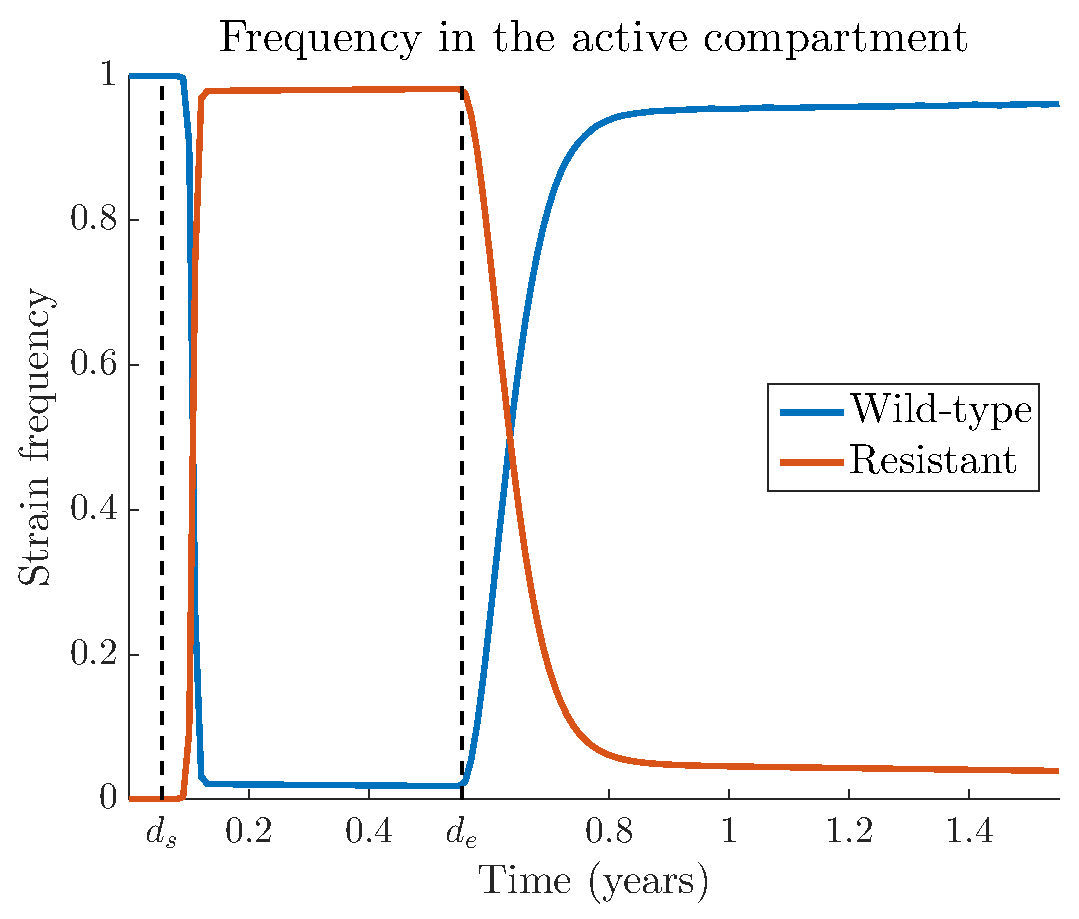
\includegraphics[width=.35\linewidth]{InfectedDynamicsActive27_06a.eps}\label{fig:sub1}}\quad%
  \sidesubfloat[]{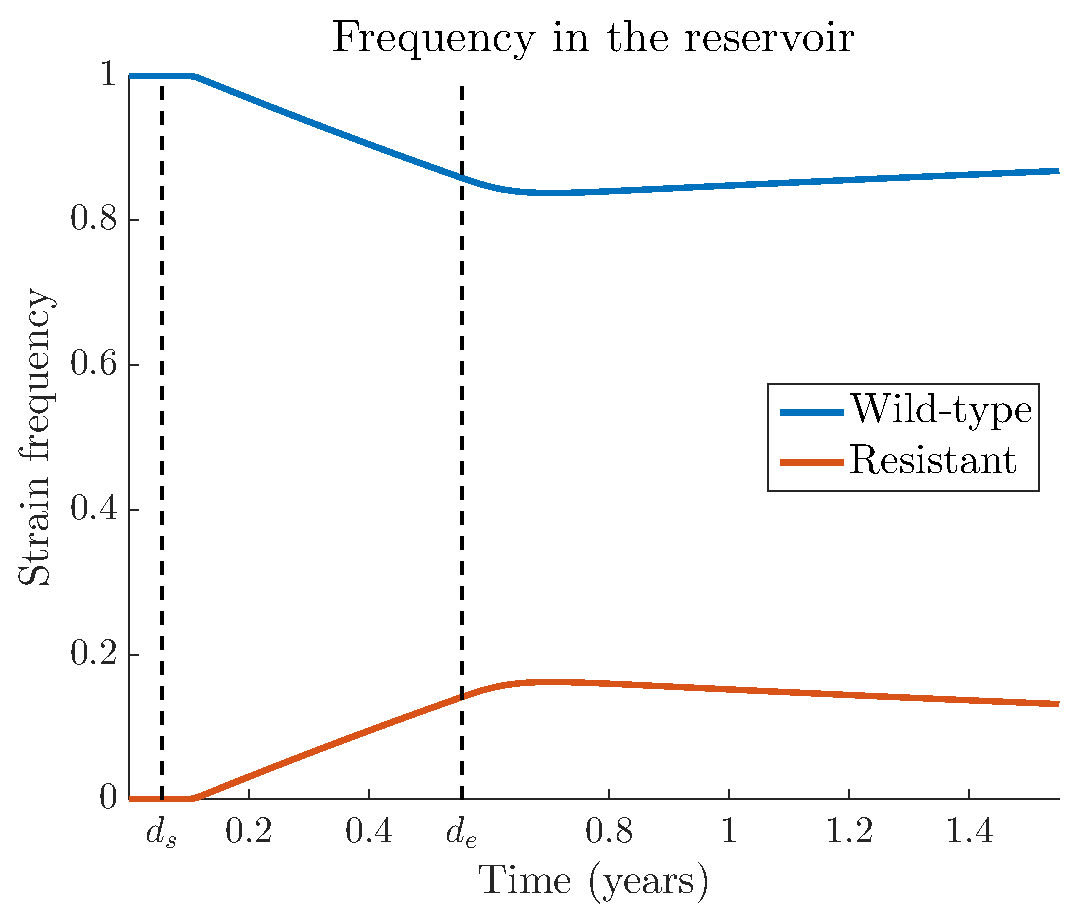
\includegraphics[width=.35\linewidth]{InfectedDynamicsRes27_06a.eps}\label{fig:sub2}}%
  \caption{The frequencies of the resistant and 
  wild-type  strains in each compartment.  The drug is administered $d_s = 20$ days after initial infection  and ends after $6$ months at $d_e$, during this time efficacy is at a maximum ($D = 1$). Where $\gamma_2=0.95$, $k=\SI{2e-3}{}$, $a = 0.01$ and $r_L = 2$. Despite a replication  rate of zero  between  $ d_s$ and $d_e$, the wild-type remains present in the active compartment due to the  large reservoir.    }\label{within host example}
\end{figure*}


The worst case scenario for the emergence of drug resistance due to PrEP is when there is a pre-existing infection(REF, many).  HIV tests are used before  administering PrEP (REF) but they are unlikely to detect the  most early stages of infection(REF)(more about tests and times?). The effectiveness of PrEP  $D(t)$ is initially chosen to reflect this. The efficacy  is zero during the first 20 days of infection (i.e. they are not on PrEP), then increases to $1$ for $6$ months at which point the treatment is stopped due to the infection(REF). 


with just prep very slowly does resistance emerge!!!  but prop with lees tann1 infections for muchtime!!

Wooiht the continnuous model resistNCE SURE TO EMERGE  BUT SINCE THIS LOW LEVEL IN POP THIS ALONE IS NOT ENOUGH TO CAUSE JEFEFHIUE

The decay of the drug once treatment  is  stopped is assumed to be exponential with a  half-life of 
$48$ hours~\cite{patterson2011}.   The  infections are assumed to be caused by a single founder strain, this is a reasonable assumption since about $80\%$ infections are found to  be caused by a single strain(REF), additionally it makes  the equations much more tractable. The reservoir can have a large impact on the frequency of  the resistant strain. 
Figure \ref{within host example} shows how the dynamics are altered with the reservoir. The host is initially infected with the wild-type strain then after $d_s = 20$ days they begin PrEP, the resistant strain soon dominates and slowly starts to fill the reservoir.  It is assumed that after $6$ months (at $t = d_e$) the infection is discovered and the treatment stopped. A longer PrEP treatment  in this case would increase the frequency in the  reservoir  further and  the slow  activation time would mean the resistant strain could be present almost indefinitely. This clearly poses a problem for the future treatment of this individual since the virus in the reservoir is only a few mutations away from being resistant to ART.










Figure \ref{within host parameter sweep} shows the frequency of resistant strain one year after PrEP  is stopped. The low levels of  drug resistance in the active compartment are consistent with experimental observations (REF); soon after PrEP is stopped resistance mutations will decrease to  very low levels(REF). Though the high mutation rate means it will not disappear entirely(REF).


%the frequncies of  the resistant strain in ht ehost are then lokee at 1 year after this ( an amount of time which may then good to do ART) and the drug decays with This may be more accurate half life for both drugs $\sim 48$h~\cite{patterson2011}.
  
  \floatsetup[figure]{style=plain,subcapbesideposition=top}
\begin{figure*}[h]
  \sidesubfloat[]{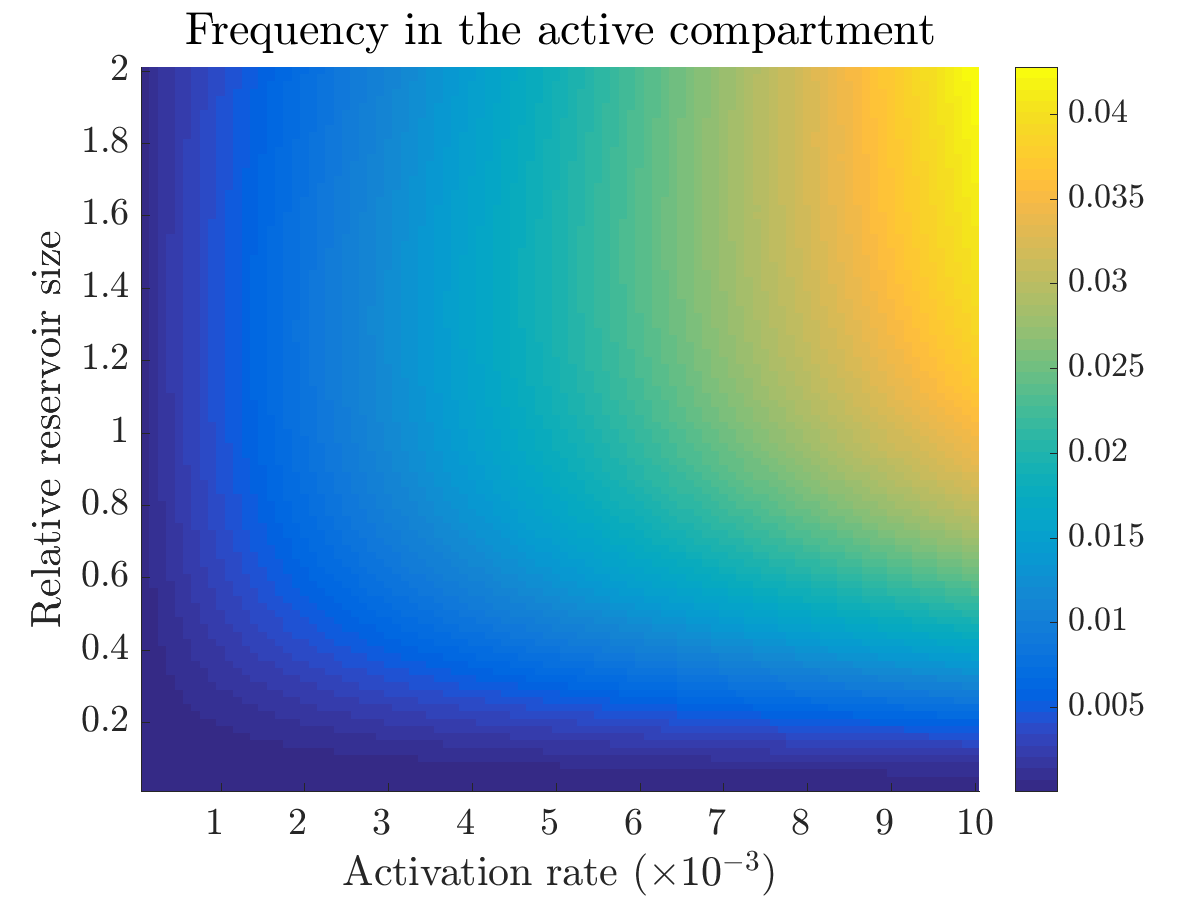
\includegraphics[width=.35\linewidth]{NoHomeo_Active_S1_Fit95_27_06a.png}\label{fig:sub1}}\quad%
  \sidesubfloat[]{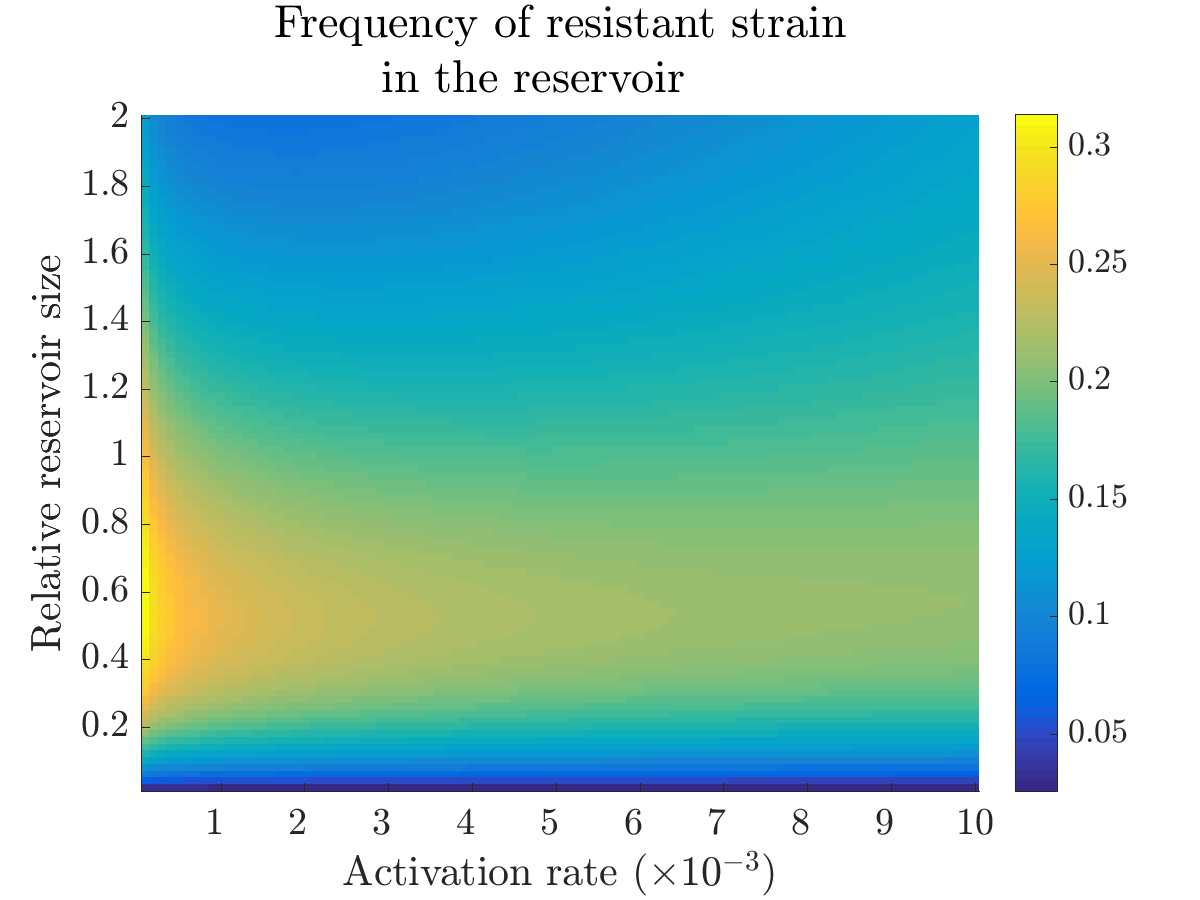
\includegraphics[width=.35\linewidth]{NoHomeo_Res_S1_Fit95_27_06a.png}\label{fig:sub2}} \\
    \sidesubfloat[]{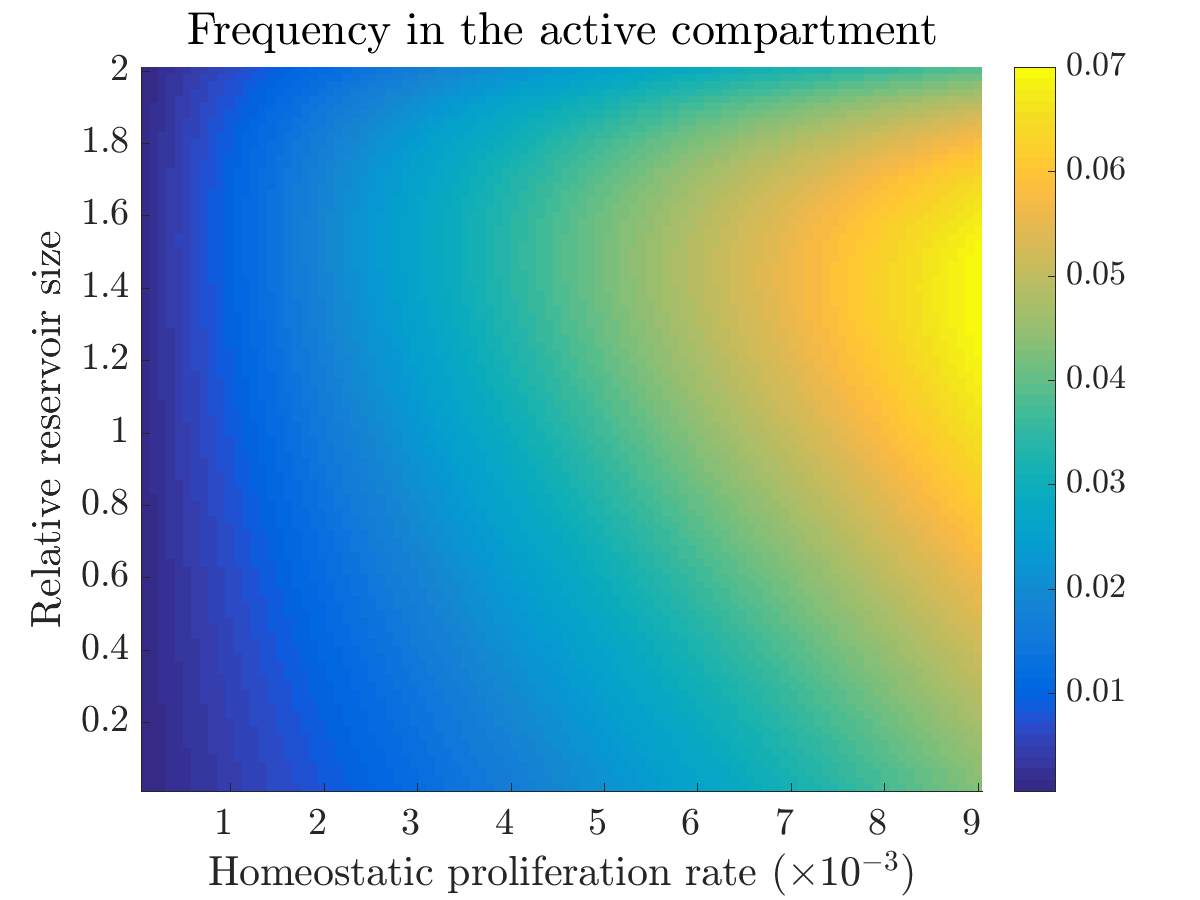
\includegraphics[width=.35\linewidth]{Homeo_Active_S1_Fit95_27_06a.png}\label{fig:sub1}}\quad%
  \sidesubfloat[]{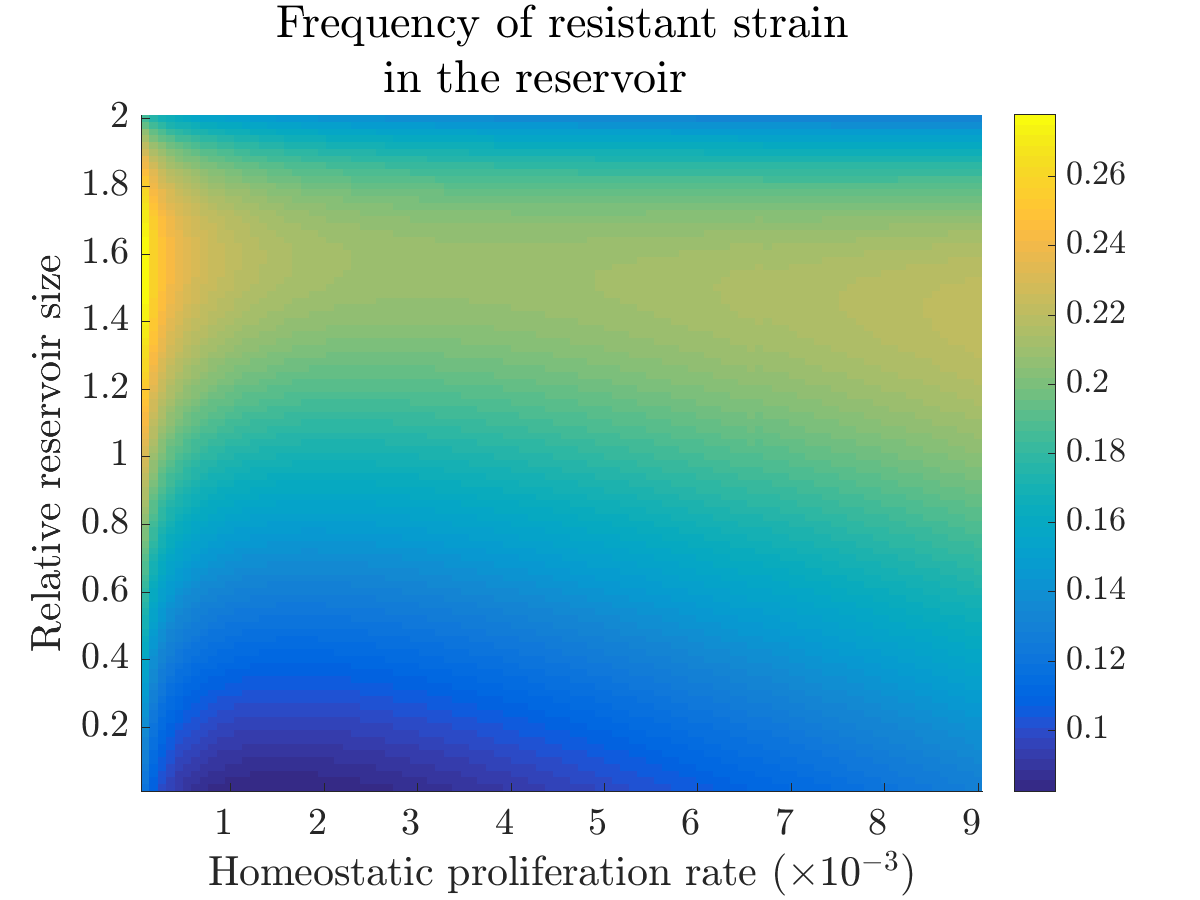
\includegraphics[width=.35\linewidth]{Homeo_Res_S1_Fit95_27_06a.png}\label{fig:sub2}}%
  \caption{The frequency of the drug resistant strain in the active and latent T cells for different parameter values one year after PrEP has stopped for a host with a pre-existing infection. (a,b) No homeostatic proliferation, i.e. $k = ar_L$. (c,d) With homeostatic proliferation and $a = 0.01$. The replication rate  of the resistant strain is $95\%$ that of the wild-type and the mutation rate is  $\SI{2.5e-9}{   }$  }\label{within host parameter sweep}
\end{figure*}



  

  
  
\subsection{between-Host Dynamics}  
 
%many of the parameters in this model will vary between individuals and my not be easy to determine...NEED THIS

Now the question is whether the resistant strain can spread through a population when PrEP use is widespread.   
There are two  main ways in which the
the use  of PrEP can lead to the development of drug resistant strains. The first, as  was mentioned above, is pre-existing infection. In various PrEP trials this was the cause of most drug  resistance. But it is a relatively infrequent occurrence, 
as many participants as  $1$ in $250$ may already be infected~\cite{iprex2011}. The second way is through poor adherence, adherence varies a great deal within and between different trials and can be low enough to render PrEP ineffective~\cite{corneli2014}. Poor adherence can increase  the  likelihood
of infection and the presence of the drug at low levels can select for resistant strains. %(though if it is too low then no).f 
Since the model is continuous resistant strains of the virus will eventually spread through the population when selected for by PrEP. But the dynamics of this can be speeded-up by poor adherence and pre-existing infections.


Initially it is assumed that $20\%$ of the population are on PrEP (i.e. $1/5$ of the susceptibles an infected individual encounters are on PrEP). Of those on PrEP $1/50$ have  pre-existing infection. It is also initially assumed that the cost associated with the wild-type infecting someone is on PrEP is $0.9$, which is consistent with the trials(REF).  All other transmission costs are set to zero. A replication rate of $ 0.95 $ is chosen for the resistant strain and a  mutation rate of $ \SI{2.5e-9}{}$ is used so that two mutations are required for resistance.
% and also kind of accounts for the compensatory mutations    
The values $\alpha_K = 1.02$ and $\alpha_{50} = 13,938$ copies per millilitre~\cite{fraser2007}  are used. Fraser \textit{et al.} (2007)  also find $\alpha_{max} = 0.317$ but a slightly larger value of  $\alpha_{max}= 0.3804$ is used (i.e. higher risk behaviour is assumed).    
 %MSM
During the acute phase of infection the maximum infectiousness is $ 3.312$. With these parameters there is a slow increase in drug resistance after the introduction of PrEP. 






 
Initially it is  assumed that  
$20\%$ of the population  go  onto PrEP at $t=0$. Of these $1$ in $40$ (??) have a pre-existing infection  and $20\%$ have poor adherence ($D(t) = 0.8$ for $ d_s \leq t \leq d_e$), with the other assumptions this allows for resistance to easily develop.




%The transmission of the virus is not simply a stochastic process; there are are several factors in the recipient host that can favour one strain over another~\cite{joseph2015}. The  exact process is not understood nd also may hve transmission from the reservoir(REF)



 %A lot of infections are found o be initiated by a single  strain, to make the model more tractable this is what is done here.


  
  %To see a reasonable impact on resistance due to PrEP $20\%$ of the population goes onto it at time $t=0$. Of these $80\%$ stick to the required doses~\cite{iprex2011,partners2012}(THIS GOOD REF?), i.e. $D(t) = 1$ for $ d_s \leq t \leq d_e$. Of these  $1$ in $250$  have a pre-existing infection~\cite{iprex2011,partners2012}(THIS GOOD REF?).
  
   
  
  \floatsetup[figure]{style=plain,subcapbesideposition=top}
\begin{figure*}[h]
  \sidesubfloat[]{\includegraphics[width=.35\linewidth]{WorstCasePop_20-06.eps}\label{fig:sub1}}\quad%
  \sidesubfloat[]{\includegraphics[width=.35\linewidth]{WorstCase_20-06.eps}\label{fig:sub2}}%
  \caption{Solution to equations(\ref{between host eqns1}-\ref{between host eqns4}). PrEP is introduced at $t=0$, there is a decrease in the number  of infections (COMPARE TO REAL).  But  the relative incidence of resistant virus increases massively during the $20$ years following introduction of PrEP.  }\label{worst case}
\end{figure*}


  


Figure  \ref{worst case} shows the between-host dynamics when all of these assumptions are made.  Before the introduction  of PrEP the relative incidence of  the resistant strain is $\sim 0 $. %2.6359e-05
During the $20$ or so years following the introduction of PrEP it reaches $\sim 0.52$.% 0.5226 
%The overall  incidence is decreased by about   which is noice  Wiht more people  on PreP even worse. But don't worry. Look now at the assumptions that were made.  First the fitness  and mutation rates   further prep will impact the replicative capacity in host omn prep 
 
The replication rate of $0.95$ for the resistant strain is likely  too high (REF) especially since  the drug has no affect on its replicate rate. Figure \ref{mutationreplication} shows that a small  decrease in the replication rate has a large impact on the relative incidence of the resistant strain.


  \floatsetup[figure]{style=plain,subcapbesideposition=top}
\begin{figure*}[h]
  \sidesubfloat[]{\includegraphics[width=.35\linewidth]{RepMUtTotalIncidence_21-06a.png}\label{fig:sub1}}\quad%
  \sidesubfloat[]{\includegraphics[width=.35\linewidth]{RepMUtIncidence_21-06a.png}\label{fig:sub2}}%
  \caption{Equilibrium values of the relative incidence for the resistant strain 
	and the total incidence. Decreasing the 
replicative capacity of the resistant strain rapidly decreases the number of  infections it can cause.	The mutation rate has a less noticeable effect.  }\label{mutationreplication}
\end{figure*}





The second important factor  is the transmission rate, it is assumed to be the same for either strain and then modified by the constants $c_{ik}^{(jl)}$. But several studies have shown that strains that are resistant to tenofovir or emtricitabine  are much less transmissible~\cite{cong2011,chateau2013,drams} compared to the wild-type. But this is only for transmission to a host not on PrEP, it is here hypothesised that it may be more transmissible (due to  competition) when the recipient is  on PrEP. As Figure \ref{cost} shows, the additional cost drastically reduces the incidence of resistant virus.  
  
  
  \floatsetup[figure]{style=plain,subcapbesideposition=top}
\begin{figure*}[h]
  \sidesubfloat[]{\includegraphics[width=.35\linewidth]{CostsTotalIncidence_21-06a.png}\label{fig:sub1}}\quad%
  \sidesubfloat[]{\includegraphics[width=.35\linewidth]{CostsIncidence_21-06a.png}\label{fig:sub2}}%
  \caption{ Equilibrium values of the relative incidence for the resistant strain 
	and the total incidence.  The cost of transmission for  the  resistant virus to  hosts on PrEP and not on PrEP, a small cost is needed  to maintain high levels of incidence.  }\label{cost}
\end{figure*}


 The parameters that  less is known about relate to  the reservoir and what is transmitted during early early infection.  Figure \ref{efjnefnje} shows  that the reservoir too has a significant  impact on the incidence of resistant infections.  It is also worth noting that the reservoir parameters ($a$,  $k$, $r_L$) that maximise incidence for one value of $tr$ will not maximise it  for another. It can be seen in Figure \ref{within host parameter sweep} that the two  compartments  are different.
  
  

 
  \floatsetup[figure]{style=plain,subcapbesideposition=top}
\begin{figure*}[h]
  \sidesubfloat[]{\includegraphics[width=.35\linewidth]{transrLTotalIncidence_21-06a.png}\label{fig:sub1}}\quad%
  \sidesubfloat[]{\includegraphics[width=.35\linewidth]{transrLIncidence_21-06a.png}\label{fig:sub2}}%
  \caption{  Equilibrium values of the relative incidence for the resistant strain 
	and the total incidence when the proportion of virus  transmitted from the reservoir and the relative size of the reservoir are changed. }\label{efjnefnje}
\end{figure*}


  
\section{discussion}  
  
  
  The  results of this numerical  model  are consistent with other models that have looked at emergence of drug resistance due to PrEP~\cite{abbas2013}(MORE) \url{http://ofid.oxfordjournals.org/content/early/2016/06/16/ofid.ofw125.full.pdf}? The use of PrEP is likely to cause a small  increase the incidence of drug resistance
  %  but not to such an extent that it would outweigh the benefits in reduced number of infections.
   The incorporation of the within-host dynamics has highlighted  how much resistant virus could potentially be stored in the latent reservoir. Even if this is unlikely to be transmitted  to another host it still represents a great danger to someone going onto ART since the virus in the reservoir may be only a few mutations away from being fully resistant to ART. If there is also transmission from the reservoir this  can  make a big difference. This also depends strongly on the early transmission events about which not much is known. If resistant virus proves to be more infectious to people on PrEP than thought or if latent cells are more important in early infection (REFS)  then there may be need for  greater concern.
   
 
  
  \iffalse
  
  
  
\subsection{Parameters}
\label{Parameters}


 This may be more accurate half life for both drugs $\sim 48$h~\cite{patterson2011}
 
 

some stuff for the hill function~\cite{shirreff2011}
~\cite{hollingsworth2008}



The values of $a$, $k$ and $r_L$ are not easy to determine (REF HIV reservoir paper)
and will also vary between individuals (REF). The relative reservoir size is estimated to be between $0.06$ and $3.1$ (REF HIV reservoir). There is more data on the replication rates and mutation rate (although still with much variation) (REF)

The two main resistance mutations for truvada and emtrabiticite are due to point mutations (REF, need this?). Mutations from one strain to another are assumed to happen at a rate of $\SI{5e-5}{}$ per replication cycle~\cite{gao2004}. This is in the range of values for which point mutations occur reasonable~\cite{abram2010}
although could be much higher depend on method~\cite{cuevas2015}(vivo) much variation also depend on vitro vivo

in any case with this rate  and high viral load all possible single mutations can happen many many times~\cite{coffin1995}

The mutations that confer resistance to the PrEP have a big impact on the fitness of these strains(REF), although there is much variability in reported stuff(REF) and also there can be compensatory mutations etc.


Elucidate the problem posed by the reservoir when drug resistance develops. The  most likely situation in which resistance will develop is  if  the PERSON has an undetected HIV infection before starting PrEP (REF iprex and partner and prob loads of  other stuff). The efficacy profile of the drug is assumed to be as in Figure \ref{Drug efficacy}. The PERSON begins taking PrEP $36$ days after being infected and then stops when the infection is detected after $6$ months (mention pharmkokinetics), one year the cessation  of PrEP the frequencies are found. varying the parameters $\rho$, $a$ and $r_L$ 
gives different results as shown in Figure \ref{within host parameter sweep}. The reservoir can contain a significant amount of the resistant strain when it has all   but disappeared in the active compartment.

assume for the figure that infection begins 
$20$ days before the PrEP (enough time for resistant strain to get S HIGH AS IT WILL  FROM MUTATION 	)  and then will  increase with PrEP, stop again  after 0.5  years then wait a year after that and see how much etc...      would expect resistancetonot be much due to  reversion but in the reservoir much more can persist see the figgreur
see that resistant strain is negligible in ctive compartment when replication  is quite high but can still  represent about $10\%$ in the reservoir for different parameters notsure  what go 

two  probs this may represent  SIGNIFICANT AMOUNT 	of latent virus thta could promote resistance in someone on ART (suggests wating longer to giving ART would be good but then peson is  more  infectious) obvs it will  decrease the proportion of resistant infections @@? because there will be more  WTs  but does  this mean there will be less in absolute terms ?



%so prob to ask is why given that resistant is there whyit not get transmitted so easily(in host competition)? in a  day  

%nonsynonomuos mutations fitness cost less than $10\%$ (ReF, need this bit?) 












%Assume small finess difference (reoplication rate, despite all the stuff from before ) and 



\subsection{Results}
Elucidate the problem posed by the reservoir when drug resistance develops. The  most likely situation in which resistance will develop is  if  the PERSON has an undetected HIV infection before starting PrEP (REF iprex and partner and prob loads of  other stuff). The efficacy profile of the drug is assumed to be as in Figure \ref{Drug efficacy}. The PERSON begins taking PrEP $36$ days after being infected and then stops when the infection is detected after $6$ months (mention pharmkokinetics), one year the cessation  of PrEP the frequencies are found. varying the parameters $\rho$, $a$ and $r_L$ 
gives different results as shown in Figure \ref{within host parameter sweep}. The reservoir can contain a significant amount of the resistant strain when it has all   but disappeared in the active compartment.





pre-infection not so common in iPREX (2 in 1251) (REF obvs) standard antibody test not find the infection 
mucu  ?? different??
more resistance reported in some tests \cite{lehman2015} this is partners 

seeing as I don't have fitness cost to resistant one in presence of drug perhaps it is best to just look at pre-existing infections

10 out of 2499 infected at enrolment~\cite{iprex2011}
100 infected at follow up (2 in the PrEP group the rest in the placebo)

in \cite{partners2012} 14 infected at start out of 4747 (would expect this to be less/more? since this is the partners study, focus more on MSM)

frequencies aas low as $1\%$ can lead to treatment failure (this mean less than this not?) some amountof resistant ok? since also done in by the drug

preexisting resistant
variants at frequencies $>1\%$ were associated with risk for virological
failure in treatment-experienced patients~\cite{boltz2011}. Does this mean that less than 1 is no problem as it says in~\cite{lehman2015}

resistance predominantly due to existing infection~\cite{lehman2015}(not good ref?)

want to maximise infectiousness over time so average?
worst case etc pere 

assume for the figure that infection begins 
$20$ days before the PrEP (enough time for resistant strain to get S HIGH AS IT WILL  FROM MUTATION 	)  and then will  increase with PrEP, stop again  after 0.5  years then wait a year after that and see how much etc...      would expect resistancetonot be much due to  reversion but in the reservoir much more can persist see the figgreur
see that resistant strain is negligible in ctive compartment when replication  is quite high but can still  represent about $10\%$ in the reservoir for different parameters notsure  what go 

two  probs this may represent  SIGNIFICANT AMOUNT 	of latent virus thta could promote resistance in someone on ART (suggests wating longer to giving ART would be good but then peson is  more  infectious) obvs it will  decrease the proportion of resistant infections @@? because there will be more  WTs  but does  this mean there will be less in absolute terms ?





\begin{figure*}
 \begin{center}$
 \begin{array}{cc}
 \includegraphics[width=.35\linewidth]{NoHomeo_Active_S1_HigFit075_09_06b.png} &
 \includegraphics[width=.35\linewidth]{NoHomeo_Reservoir_S1_HigFit075_09_06b.png} \\
  \includegraphics[width=.35\linewidth]{Homeo_Active_S1_HigFit075_09_06b.png} &
 \includegraphics[width=.35\linewidth]{Homeo_Reservoir_S1_HigFit075_09_06b.png}
 \end{array}$
 \end{center}
 \caption{The frequency of the drug resistant strain in the active and latent T cells for different parameter values. (a,b) In the absence of homeostatic proliferation this happens i.e. $k = ar_L$ . (c,d) with homeostatic prliferation and $a = 0.01$.  drug as in druf 
 The fitness of the resistant strain is $75\%$ that of the wild-type. the fitness chagnes  the speed  of the stuff but the values is the same  }
 \label{within host parameter sweep}
 \end{figure*} 

As is seen experimentally (REF) in the absence of the resistant drug the resistant strain soon diminishes,  for the parameters considered here the frequency of resistant strain in the active T cells (compartment) is very low, but there is much more range of values for the resistane strain in the reservoir. A potetntial risk for development 
of resistanecce, based on this transmission from resistant in active compartment not so muchfo a problem,  but what about when strains come from the reservoir either during ART or prefferntial transmission, but also  range of parameters for these two things to happen not the same. So there is potential for the resistant strain to hang around longer than we think, but how easily can it be transmitted, experiments have shown that resistant strains are not so transmissible (REF) due to decreased fitness.  But what if they get into someone on PrEP do they have an advantage in within host competition? Already said that HIV in reservoir persists for ever so going ontp ART with this may be a problem

values different in the presence of  homeostatic proliferation larger reservoir will make more resistane t
 no home a =0 is no reservoir

MSM??




$$how quick viral load go back up after no more PrEP$$

The reservoir can have 


\section{between host stuff}
   \subsection{parameters}
biggest danger is pre-existing infections but these are not so common


  
USE THIS
To enable comparison between the models, each model
simulated two strategies over 20 years: In the first strategy,
ARTwas provided, and in the second strategy, both PrEP
and ARTwere provided. The key outputs of the models
for comparison were the prevalence of HIV in the general
population, the prevalence of HIV drug resistance in
the general population, the proportion of infected
individuals with resistant infections and the source of
drug-resistant infection.


\section{09/06}
non/low adherance relatively the same as preexisting infection for how many infections they casue, this when effectiveness is at $ 80\%$
Inmodel what makes difference 

transmissibility and fitnessof resistant strain, data mostly show this to be low.  for more complex transmission assumptions(preferential also maybe???) reservoir will likely impact and also for future art use.What parameter is biggest danger. Also obviously different amounts of non-adhering and moreprep users will have impact. Get transmission stuff fixed then go over all these and see what is the worst

 
 
 for between ohst assume about a $75\% $ drop in transmisibility for WT~\cite{partners2012}
 
 
 
 
 \section{What you do}
 
nedd functionto lower transmssibiilty reltive to WT or  something. increase tranmsisibilyof and decrese the other n presenc of  the drug to  simulate the competiton 

AHHH
reduce WT TRANSMISSIBILITY BY  a lot  and also reduce/increase for resistant. Will this ccount for differences in numbers not explicity doing any competition though
For  lower VL strain fitness may be more important but at higher levels more stochastic? Or the other way round?
 
 probably only change infectivity during acute phase.
 


\section{copetition}
 majority of infectionsresult of a singel founder strain (REF). Howthis happens not entirely clear, with in the genitla tract there are several mechaisms which can influence the spread~\cite{joseph2015} and also vl heritability~\cite{fraser2014}
 
 Aslo the concentration of the drug is not the same throught th body~\cite{patterson2011}
 
 
 \section*{VL and transmissibilty}
 
saturation of transmissibility for high viral loads~\cite{fraser2007}, so for large enough amounts of virus. For  ACUTE PHASE JUST ASSSUME  	infectiousness  is  proportionalto frequency since there is  so much (right?). For  high vl infectiousness not change much, VL of WT on PrEP has max, i.e. when you on PrEP the VL is reduced 
 
 
 
 \section*{write up}
 
\begin{enumerate}
\item intro 1-2 k words all about HIOV PrEP impportance ...
\item Methods short initial description, 1.5k total
\begin{enumerate}
\item within host. Equations and parameters jusstifiedand explained,

\item between host. infectivity all  this with the hill function and parameters and justify 



\end{enumerate}

\item results. 1.5k words
\begin{enumerate}
\item within host.  pic of paramter sweep and oooh time  to ART important 


\item between host. 

\end{enumerate}
\item discussion .5k words
\end{enumerate} 
 
 
 
 
 AAAAAAAAAAAAAA
   increasing tim to art means thers is time to make more resistant infeciont but also pose less threat to art and gif time for 
   
   
   blt mice \url{http://journals.plos.org/plosmedicine/article?id=10.1371/journal.pmed.0050016}
 
 
 \fi
 
 
 
 
%\begin{acknowledgements}
%If you'd like to thank anyone, place your comments here
%and remove the percent signs.
%\end{acknowledgements}

% BibTeX users please use one of
\bibliographystyle{spr-chicago}      % Chicago style, author-year citations
\bibliography{DTCProject1Bibliography}   % name your BibTeX data base
\nocite{*}



\end{document}
% end of file template.tex


 
 
 \iffalse
 
\bibliographystyle{spr-chicago}
\bibliography{DTCProject1Bibliography} 


 
\end{document}



\fi
